% Created 2016-12-18 Sun 21:07
\documentclass[10pt,conference,compsocconf]{IEEEtran}
\usepackage[utf8]{inputenc}
\usepackage[T1]{fontenc}
\usepackage{fixltx2e}
\usepackage{graphicx}
\usepackage{grffile}
\usepackage{longtable}
\usepackage{wrapfig}
\usepackage{rotating}
\usepackage[normalem]{ulem}
\usepackage{amsmath}
\usepackage{textcomp}
\usepackage{amssymb}
\usepackage{capt-of}
\usepackage{hyperref}
\usepackage{bm}
\usepackage{svg}
\usepackage{graphicx}
\graphicspath{{pics/}}
\usepackage[margin=1in]{geometry}
\usepackage{algorithm}
\usepackage{algpseudocode}
\documentclass[10pt,conference,compsocconf]{IEEEtran}
\author{Laurent Lejeune, Tatiana Fountoukidou, Guillaume de Montauzon}
\date{\today}
\title{Group 97: Road Segmentation}
\hypersetup{
 pdfauthor={Laurent Lejeune, Tatiana Fountoukidou, Guillaume de Montauzon},
 pdftitle={Group 97: Road Segmentation},
 pdfkeywords={},
 pdfsubject={},
 pdfcreator={Emacs 25.1.1 (Org mode 8.3.6)}, 
 pdflang={English}}
\begin{document}

\maketitle


\section{Related works}
\label{sec:orgheadline6}
\subsection{Road Segmentation in Aerial Images by Exploiting Road Vector Data \cite{6602035}}
\label{sec:orgheadline1}
\subsection{Morphological road segmentation in urban areas from high resolution satellite images \cite{gaetano:inria-00618222}}
\label{sec:orgheadline2}
\subsection{Connected Component-Based Technique for Automatic Extraction of Road Centerline in High Resolution Satellite Images \cite{sujatha15_connec_compon_based_techn_autom}}
\label{sec:orgheadline3}
\subsection{Machine Learning Based Road Detection from High Resolution Imagery}
\label{sec:orgheadline4}
\subsection{Road Extraction Using K-Means Clustering and Morphological Operations \cite{maurya2011road}}
\label{sec:orgheadline5}

\section{Data exploration}
\label{sec:orgheadline7}
The provided training set contains 100 images of size 400x400 along with their ground-truth. A total of 6 images are discarded because they either show a too small quantity of positive class pixels, or some misleading regions such as rail-tracks. 
We notice that most images are made of grid-like roads, sometimes occluded by trees. 
\section{Mid-level segmentations}
\label{sec:orgheadline8}
The image pixels are first grouped in two different manners:
\begin{enumerate}
\item Square patches: The image is divided in non-overlapping patches of size 16x16.
\item SLIC Superpixels (Simple Linear Iterative Clustering) \cite{achanta12}: Pixels are grouped in mid-level regions in an iterative manner. The algorithm starts from a regular grid of cluster centers and iteratively updates the labels of their neighboring centers based on a distance measure. This method improves over the square patches method because the pixels are already pre-segmented. Their feature vector will therefore be easier to discriminate.
\end{enumerate}
\section{Feature extraction}
\label{sec:orgheadline9}
Following an exploration of the related litterature, we select a set of features to extract.
\begin{itemize}
\item SIFT (Scale-Invariant Feature Transform) \cite{lowe99}: This descriptor is used extensively in computer-vision applications. It computes a histogram of oriented gradients on 16x16 windows centered at a keypoint and gives a descriptor of 128 scalar values. The keypoint detection step is not performed, instead we extract the descriptors on a dense grid at canonical scale and orientation. As advised in \footnote{\url{https://people.csail.mit.edu/hasinoff/320/sift-notes.txt}

\bibliographystyle{ieeetr}
\bibliography{refs}
\printbibliography} to improve illumination invariance, the integer value descriptors are first normalized to unit-norm, ceiled to 0.2, and renormalized to unit-norm. As we require that each segment be represented by a single feature vector, we encode the dense SIFT descriptors contained in a given segment in a "bag-of-features" manner through the following steps: 
\begin{enumerate}
\item Based on a sufficiently large number of SIFT descriptors computed on 10 images, we start by fitting a PCA model. We have checked that the explained variance at 60 components is above 99\%.
\item A codebook is generated on the aforementioned training samples. A codebook is merely a set of K-means clusters that is used to encode the input (compressed) descriptors to integer values.
\item We then compute a normalized histogram of codes (bag-of-features) in each segment. This gives us a single texture feature vector for mid-level regions.
\end{enumerate}
\item Hough line transform: This transformation has already been used in a state-of-the-art method \cite{2016ISPAr41B3..891L}. First, the edge map is computed using a canny edge detector. Given some parameters, a set of lines are extracted on the edge maps and sorted based on their RGB variance, i.e. we want to keep the lines along which the color variations is minimal. An example is shown on figure \ref{fig:orgparagraph1}. As feature, we take the mean value of the hough map on the segment.
\item Euclidean distance transform. This straightforward transform is used to compute, at each pixel location, the shortest "taxicab" distance to an edge pixel. Using as input the canny edge map, we expect this feature to discriminate cluttered regions such as those containing blocks of buildings where the Euclidean distance tends to be smaller. The mean value over the segment is used.
\item Mean RGB value. Roads tend to have greyish colors.
\end{itemize}
To summarize, our feature extraction procedure provides a total of 65 features per superpixel.

\begin{figure}[htb]
\centering
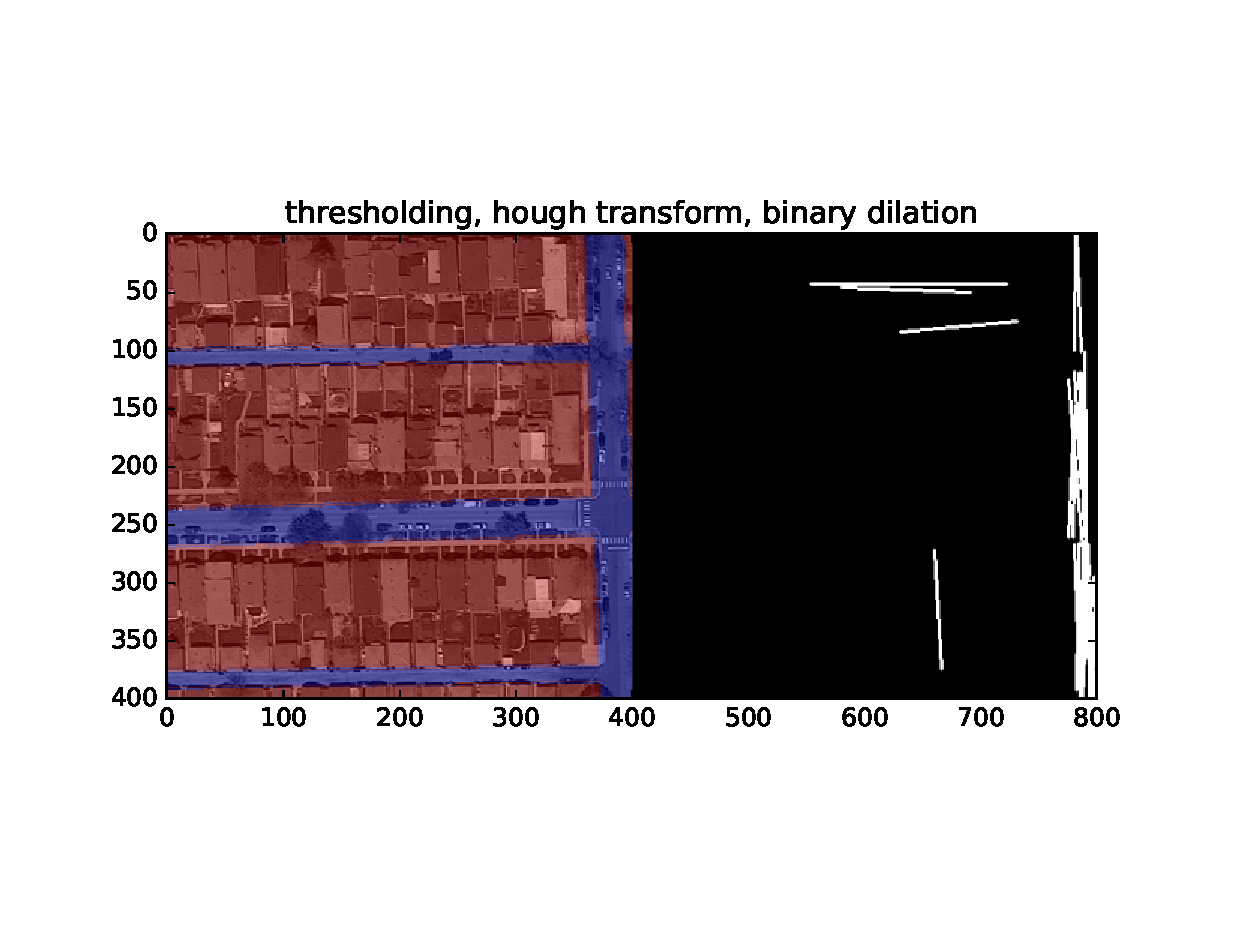
\includegraphics[width=0.5\textwidth]{pics/ex_hough.eps}
\caption{\label{fig:orgparagraph1}
Example of a hough transform. Left: Input image with the ground-truth overlay. Right: 20 lines with lowest color variance.}
\end{figure}
\section{Methods}
\label{sec:orgheadline12}
Two (several) methods have been implemented and tested. A structured model will provide a baseline. It will be compared to a Convolution Neural Network approach.
\subsection{Refinement of generic models using structured SVM}
\label{sec:orgheadline11}
\begin{figure}[htb]
\centering
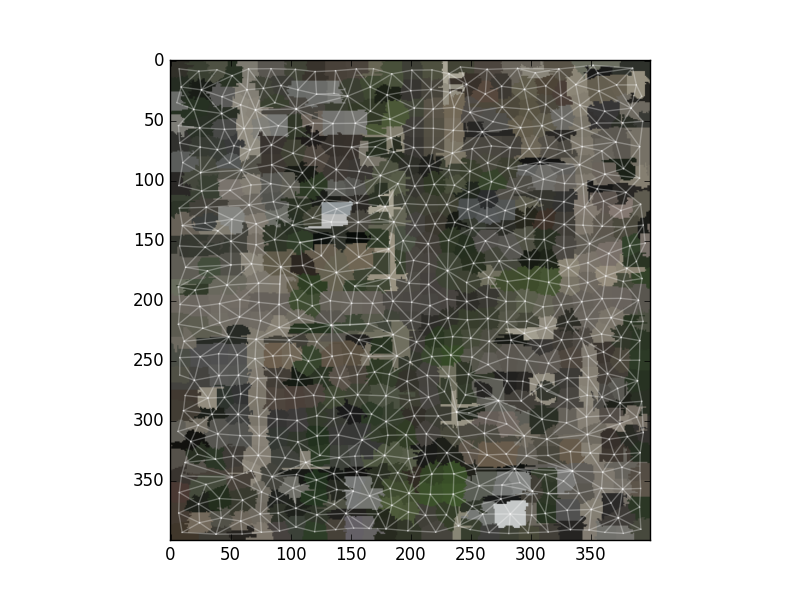
\includegraphics[width=0.5\textwidth]{pics/ex_graph.png}
\caption{\label{fig:orgparagraph2}
Example of a superpixel-segmented image with connecting edges.}
\end{figure}

   Using structured models \cite{tsochantaridis05}, one can leverage the spatial relations between mid-level regions. As shown on figure \ref{fig:orgparagraph2},a segment considered as road gives a strong prior on the "roadness" of its neighboring segment. This is formalized as an undirected graph on which the node features are assigned unary potentials. In our case, the unary potentials are given by probability estimates given by generic models such as logistic regression or random forest.
Inspired by \cite{fulkerson09}, the edge costs are made off of two features: The difference in mean LUV color, and the number of pixels that separate two segments (length of separating path). This last feature allows to penalize segments that are "weakly" connected. Indeed, we have verified visually that roads tend to be composed of regular chains of square-like segments, thereby justifying that choice.

Formally, structured models aim at maximizing an energy functions of the form:

 \begin{equation}
 \begin{split}
E_w(X,Y) &= \sum_{i \in \mathcal{V}} E_{data}(y_i;x_i) + \sum_{i,j \in \mathcal{E}} E_{smooth}(y_i;y_j) \\
 &= \mathbf{w}^T \psi(X,Y)
 \end{split}
 \end{equation}

Where \(\mathcal{V}\) is the set of vertices representing a segment, \(\mathcal{E}\) are the edges. The data and smoothness term are combined in the joint-features vector \(\psi\). The variable \(y\) represents the structured labels. In our setup, any probabilistic regression model (logistic regression, random forest,\ldots{}) can be used for the data term. Following \cite{fulkerson09}, the pair-wise edges potentials are given by:

 \begin{equation}
\phi(c_i,c_j|s_i,s_j) = \frac{L(s_i,s_j)}{1+\lVert s_i - s_j \rVert}
 \end{equation}
Where \(c\) and \(s\) are the mean LUV-space colors. The function \(L\) expresses the length of the shared boundaries between two segments.
\begin{enumerate}
\item Algorithm
\label{sec:orgheadline10}
The provided code relies on the pyStruct package \cite{muller14}, which implements the cutting-plane algorithm proposed by Tsochantaridis et al \cite{tsochantaridis05}.
\end{enumerate}
\end{document}